\documentclass[runningheads]{llncs}

\usepackage{amsmath,amssymb}
\usepackage{array,booktabs,float,graphicx,listings,multirow,xcolor,tikz,url}
\usepackage{longtable,capt-of,needspace,xr}
\usetikzlibrary{arrows.meta,backgrounds,fit}
\emergencystretch=1.5em

\definecolor{vanilla}{RGB}{75,105,145}
\definecolor{flexible}{RGB}{0,125,120}
\definecolor{slotblue}{RGB}{20,85,155}
\definecolor{slotorange}{RGB}{180,80,10}
\newcommand{\Tool}{\textsc{acgn}}
\newcommand{\CanDis}{\textsc{CanDis}}
\newcommand{\Seq}{\texttt{Seq}}
\newcommand{\Bag}{\texttt{Bag}}
\newcommand{\Set}{\texttt{Set}}
\newcommand{\TEmb}{\operatorname{TEmb}}
\newcommand{\TRen}{\operatorname{TRen}}
\newcommand{\EqCert}{\operatorname{EqCert}}
\newcommand{\Rep}{\operatorname{Rep}}

\newcommand{\Fix}[1]{\textcolor{blue}{#1}}

% Machine-readable paper--Lean correspondence tag.  The second argument is
% the frozen fully qualified Lean declaration name; tags are visually silent.
\providecommand{\leanref}[2]{}


\title{Typed Flexible-Arity Slotted E-Graphs:\\
Supplementary Material}
\titlerunning{Typed Flexible-Arity Slotted E-Graphs: Supplement}
\author{Anonymous Author(s)}
\institute{}

\externaldocument{main_compressed}
\begin{document}
\raggedbottom
\maketitle
This supplement accompanies the paper. Appendix~\ref{app:formal-details}
contains supporting calculations, exact Lean theorem mappings, proof
dependencies, and implementation check boundaries;
Appendix~\ref{app:evaluation-detail} gives the v3.3 results by invariant and the historical synthetic scaling study;
and Appendix~\ref{app:canon-rules} collects the rewrite policy and side
conditions. The proofs of the two main theorems and two supporting propositions
appear in the main paper.
\appendix
\section{Supporting Calculations, Lean Correspondence, and Verification Scope}
\label{app:formal-details}

The main paper proves the four core theoretical results over the abstract
formal model. This appendix provides the two elementary calculations referenced
in Sections~\ref{sec:background} and~\ref{sec:formalism}, the exact
paper-to-theorem map and proof dependency structure against the Lean~4.33.0
development at tag \texttt{v3}, the remaining formalized lemmas, and the exact
boundary between formal proofs and Java implementation checks.

\subsection{Supporting Calculations}

\paragraph{Size of binary AC closure.}
Take $n$ distinct generators with no unit or additional equations. Square-free
subproducts correspond to nonempty subsets of generators, yielding $2^n-1$
classes. An ordered binary node corresponds to a pair of nonempty disjoint
subsets: each generator is placed on the left, on the right, or in neither.
Of the $3^n$ ternary assignments, $2^n$ leave the left side empty and $2^n$
leave the right side empty, overlapping on the single all-absent assignment.
Adding that overlap back yields $3^n+1-2^{n+1}$ ordered binary nodes.

\paragraph{Changing caller names.}
Suppose two leader invocations align via
$\rho\circ\widehat m=\widehat m'\circ\pi$. After caller renamings $\eta$ and
$\eta'$, the alignment transports via conjugation
$\bar\rho=\eta'\circ\rho\circ\eta^{-1}$ because
\[
 \bar\rho\circ\eta\circ\widehat m
 =\eta'\circ\rho\circ\widehat m
 =\eta'\circ\widehat m'\circ\pi.
\]
When $\rho$ is the identity, $\widehat m=\widehat m'\circ\pi$. Because $\pi$ is
a bijection, $\operatorname{im}(\widehat m)=\operatorname{im}(\widehat m')$, so
any justified leader symmetry preserves the set of caller slots used.

\subsection{Paper-to-Theorem Map and Proof Dependencies}

Table~\ref{tab:lean-correspondence} maps each main-text result (plus the
typed-slot partitioning property underlying Section~\ref{sec:eval-synthetic})
to its exact file path and Lean declaration name(s) in the \texttt{v3}
repository. Table~\ref{tab:lean-remaining} records the remaining supporting
formal results.

\begin{table}[ht]
\centering
\caption{Paper-to-theorem map against the Lean development at tag
\texttt{v3}. Module paths under \texttt{TypedSlottedEGraphsPaper/} live in
\texttt{paper-claims/formal/TypedSlottedEGraphsPaper/}.}
\label{tab:lean-correspondence}
\scriptsize
\setlength{\tabcolsep}{2.2pt}
\begin{tabular}{@{}%
>{\raggedright\arraybackslash}p{3.0cm}%
>{\raggedright\arraybackslash}p{3.0cm}%
>{\raggedright\arraybackslash}p{5.75cm}@{}}
\toprule
Paper result & Repository file (\texttt{v3}) & Exact Lean declaration(s)\\
\midrule
Theorem~\ref{thm:shape-exactness}: Effective-support canonical-shape exactness &
\texttt{TypedSlottedEGraphs\allowbreak Paper/\allowbreak Normalization\allowbreak Bridge.lean} &
\texttt{AmbientQuotient\allowbreak Presentation.\allowbreak ambientQuotientNormal\allowbreak FormExactness},
\texttt{EffectiveSupport\allowbreak Canonicalizer.\allowbreak effectiveSupportCanonical\allowbreak ShapeExactness},
\texttt{EffectiveSupport\allowbreak Canonicalizer.\allowbreak canonicalRecord\allowbreak Postconditions}\\[4pt]
Proposition~\ref{thm:structural-soundness}: Structural realization and congruence soundness &
\texttt{TypedSlottedEGraphs\allowbreak Paper/\allowbreak StructuralContainer\allowbreak Adapter.lean};
\texttt{Structural\allowbreak Semantics.lean} &
\texttt{concreteTypedAlpha\allowbreak SemanticSoundness},
\texttt{concretePortAndNode\allowbreak CongruenceCertificate},
\texttt{concretePortAndNode\allowbreak CongruenceSemanticSoundness},
\texttt{StructuralRealizer.\allowbreak structuralRealizationNaturality},
\texttt{structuralAlphaBinderBlock\allowbreak SemanticSoundness},
\texttt{structuralPortAndNode\allowbreak CongruenceSoundness}\\[4pt]
Proposition~\ref{thm:collision-soundness}: Compatible effective-shape collisions &
\texttt{TypedSlottedEGraphs\allowbreak Paper/\allowbreak TheoremBridge.lean} &
\texttt{paperF25CertifiedLeader\allowbreak KernelExtraction},
\texttt{canonicalEqualityYields\allowbreak KernelCollision},
\texttt{paperF26CertifiedEffective\allowbreak ShapeCollision},
\texttt{paperAtom038Ambient\allowbreak CollisionCertificate}\\[4pt]
Theorem~\ref{thm:semantic-sound}: Certificate-preserving reachability and finite-unfolding soundness &
\texttt{TypedSlottedEGraphs\allowbreak Paper/\allowbreak TheoremBridge.lean};
\texttt{Reachability.lean}; \texttt{TraceSemantics.lean} &
\texttt{paperF24FindAndFinite\allowbreak UnfoldingPreserve\allowbreak EquationalCertificates},
\texttt{paperF27CertificatePreserving\allowbreak ReachabilityAndFinite\allowbreak UnfoldingSoundness},
\texttt{certificatePreserving\allowbreak ReachabilityAndFinite\allowbreak UnfoldingSoundness},
\texttt{obligationAddition\allowbreak PreservesCoherence},
\texttt{obligationRekey\allowbreak PreservesCoherence},
\texttt{obligationRemoval\allowbreak PreservesCoherence},
\texttt{obligationComposition\allowbreak PreservesCoherence}\\[4pt]
Section~\ref{sec:eval-synthetic}: Typed-slot partition search &
\texttt{docs/slot-typing-\allowbreak ablation/\allowbreak Partitioned\allowbreak Permutation.lean} &
\texttt{PartitionedPermutation.\allowbreak generated\_\allowbreak preserves\_\allowbreak key},
\texttt{PartitionedPermutation.\allowbreak generated\_\allowbreak rejects\_\allowbreak cross\_\allowbreak partition},
\texttt{PartitionedPermutation.\allowbreak every\_\allowbreak preserving\_\allowbreak mapping\_\allowbreak is\_\allowbreak represented}\\
\bottomrule
\end{tabular}
\end{table}

\begin{table}[ht]
\centering
\caption{Remaining formalized Lean results at tag \texttt{v3}.}
\label{tab:lean-remaining}
\scriptsize
\setlength{\tabcolsep}{2.2pt}
\begin{tabular}{@{}%
>{\raggedright\arraybackslash}p{2.95cm}%
>{\raggedright\arraybackslash}p{3.05cm}%
>{\raggedright\arraybackslash}p{5.75cm}@{}}
\toprule
Topic & Repository file (\texttt{v3}) & Exact Lean declaration(s)\\
\midrule
Binary AC closure counts &
\texttt{TypedSlottedEGraphs\allowbreak Paper/\allowbreak ACClosureCounts.lean} &
\texttt{ACClosureCounts.\allowbreak completeBinary\allowbreak ACClosureCounts},
\texttt{ACClosureCounts.\allowbreak sizeOfComplete\allowbreak BinaryACClosure}\\[3pt]
Category, support, rebuild quiescence &
\texttt{TypedSlottedEGraphs\allowbreak Paper/\allowbreak StructuralClaims.lean} &
\texttt{typedEmbedding\allowbreak CategoryLaws},
\texttt{leaderization\allowbreak ContractsSupport},
\texttt{finiteRebuildQuiescence}\\[3pt]
Concrete support and invocation safety &
\texttt{TypedSlottedEGraphs\allowbreak Paper/\allowbreak SyntaxSupport.lean} &
\texttt{concreteTypedEmbeddings\allowbreak PreserveTypes},
\texttt{concreteSlotSupportInvariance},
\texttt{concreteTypeSafety\allowbreak OfInvocation}\\[3pt]
Parent forest and collision index &
\texttt{TypedSlottedEGraphs\allowbreak Paper/\allowbreak ContextGraph.lean} &
\texttt{FiniteTypedParentForest.\allowbreak find\_\allowbreak support\_\allowbreak contracts},
\texttt{QuiescentFiniteTypedEGraph.\allowbreak graphInvocation\allowbreak Alignment\_\allowbreak transport},
\texttt{QuiescentFiniteTypedEGraph.\allowbreak identityAligned\allowbreak LeaderSupport},
\texttt{F10FiniteQuiescentGraph\allowbreak Environment.\allowbreak collisionIndexExact}\\[3pt]
Source rule laws and arithmetic profile &
\texttt{TypedSlottedEGraphs\allowbreak Paper/\allowbreak ProfileRules.lean} &
\texttt{tsgRule012\_\allowbreak phaseLocalPrenex\allowbreak AndDomainGuarding}--\texttt{tsgRule019\_\allowbreak implicationLocalSaturation},
\texttt{tsgCe003\_\allowbreak overflowReassociation\allowbreak Counterexample},
\texttt{tsgScope001\_\allowbreak zeroCanonical\allowbreak DistanceBoundary}\\[3pt]
Worked abstract trace witness &
\texttt{TypedSlottedEGraphs\allowbreak Paper/\allowbreak TraceEnvelope\allowbreak Witness.lean} &
\texttt{TraceEnvelopeWitness.\allowbreak d1\_\allowbreak trace\_\allowbreak obligation},
\texttt{TraceEnvelopeWitness.\allowbreak d2\_\allowbreak trace\_\allowbreak obligation},
\texttt{TraceEnvelopeWitness.\allowbreak machineChecked\allowbreak EndToEndWitness}\\[3pt]
Slot-typing grid \& negative controls &
\texttt{docs/slot-typing-\allowbreak ablation/\allowbreak Model.lean}, \texttt{BalancedGrid.lean}, \texttt{Independent\allowbreak BindingBlocks.lean} &
\texttt{different\_\allowbreak sorts\_\allowbreak distinct}, \texttt{erasure\_\allowbreak can\_\allowbreak collide},
\texttt{typed\_\allowbreak mappings\_\allowbreak subset}, \texttt{allocation\_\allowbreak total}, \texttt{balanced},
\texttt{mixed\_\allowbreak quantifier\_\allowbreak exchange\_\allowbreak is\_\allowbreak invalid},
\texttt{dropping\_\allowbreak disjointness\_\allowbreak is\_\allowbreak invalid},
\texttt{moving\_\allowbreak all\_\allowbreak across\_\allowbreak eventually\_\allowbreak is\_\allowbreak invalid}\\[3pt]
Source normalization scheduling &
\texttt{docs/distance-parity-\allowbreak 20261107/\allowbreak CapabilitySource\allowbreak Scheduling.lean} &
\texttt{membership\_\allowbreak before\_\allowbreak distribution},
\texttt{subcarrier\_\allowbreak membership\_\allowbreak elimination},
\texttt{restriction\_\allowbreak universal\_\allowbreak neutral},
\texttt{empty\_\allowbreak domain\_\allowbreak guard\_\allowbreak retained},
\texttt{disjoint\_\allowbreak declarations\_\allowbreak retained}\\
\bottomrule
\end{tabular}
\end{table}

\paragraph{Module dependency structure and trusted computing base.}
The main formal development under \texttt{paper-claims/formal/} has an acyclic
module graph:
\begin{quote}\small
\texttt{Core} $\to$ \{\texttt{SyntaxSupport}, \texttt{ContextGraph},
\texttt{Certificates}\}\\
$\to$ \{\texttt{FiniteNormalization} $\to$ \texttt{NormalizationBridge},\\
\hspace*{1.2em}\texttt{StructuralSemantics} $\to$ \texttt{StructuralContainerAdapter},\\
\hspace*{1.2em}\texttt{TraceSemantics} $\to$ \texttt{Reachability}\}\\
$\to$ \texttt{TheoremBridge} $\to$ \texttt{ClaimLedger} / \texttt{PaperIndex}.
\end{quote}
Across the audited Lean~4.33.0 development (\texttt{tcb-manifest.json}
under \texttt{paper-claims/formal/}),
the 146 active mapped units depend solely on Lean's standard foundational
axioms (\texttt{propext}, \texttt{Quot.sound}, \texttt{Classical.choice}),
with zero project-defined axioms, zero \texttt{sorry} placeholders, and zero
\texttt{native\_decide} or unsafe dependencies.

\subsection{Formal Proofs vs.\ Implementation Checks and Empirical Evidence}

To keep formal and empirical claims distinct:
\begin{itemize}
\item \textbf{Formal-model theorems} (Table~\ref{tab:lean-correspondence})
  establish exactness, realization soundness, collision soundness, and
  coherence-preserving finite-unfolding soundness over the Lean abstract
  model, plus one concrete machine-checked abstract trace in
  \texttt{TraceEnvelopeWitness}.
\item \textbf{Java implementation checks} consist of (i)~in-process
  strict-every-transition invariant and certificate checks in
  Certificate-Integrated IR, (ii)~an independent Java certificate verifier and
  adversarial suite covering support contraction, collision, union, symmetry,
  rebuilding, path compression, container laws, binder orbits, and incomplete
  evidence, (iii)~the native-operation comparison across all 61,598 eligible
  paired comparisons (0 mismatches, 0 unchecked, 0 invalid replays, 0 errors),
  and (iv)~bounded Alloy checks on the union of 4,499 natural zero claims and
  29 capability subtype checks.
\item \textbf{Open verification boundary:} The native-operation comparator
  authenticates its \texttt{FROZEN\_NORMALIZED\_IR} boundary, while general
  Java-to-Lean correspondence (\texttt{javaLeanCorrespondence\allowbreak Checked}),
  source-to-certificate wire replay (\texttt{sourceCertificateWire\allowbreak ReplayChecked}),
  and public repair-sequence linkage (\texttt{publicSequenceLinked}) remain
  open. Likewise, observed zero-discrepancy agreement between Fast Rewrite and
  Certificate-Integrated IR is an empirical check on the evaluated workloads,
  not a universal equivalence theorem.
\end{itemize}

\paragraph{Source rewrites added in v3.1.}
In \path{docs/section3-repair-audit/formal/Phase5SourceRules.lean},
\path{unary_restrictions_are_intersection} treats unary restrictions, and
\path{unary_image_of_domain_restriction} handles the typed join boundary.
\path{static_all_commutes_with_always} fixes the domain across time;
\path{changing_domain_blocks_all_always} refutes the unrestricted law.
\path{next_fixed_binding_observation} keeps the bound value fixed and primes
the observed carrier. The subdomain and difference lemmas restrict the
binding at its original instant. These are results about the formal source
semantics, not a proof of the whole Java frontend.

\clearpage
\section{Experimental Detail}
\label{app:evaluation-detail}

The following appendix preserves the v3.3 natural-corpus, reference-pool,
runtime and capability tables and by-invariant plots from 26 November 2026.
The current measurements are in Section~\ref{sec:evaluation}. The synthetic
scaling study comes from v3 and retains its 300-second deadline.

\subsection{Pipeline Variants}

\begin{table}[H]
\caption{Representation and equality discovery across the five distinct
baselines and the two \CanDis{} implementations.}
\label{tab:engine-boundary}
\centering
\scriptsize
\setlength{\tabcolsep}{3pt}
\begin{tabular}{@{}%
>{\raggedright\arraybackslash}p{2.45cm}%
>{\raggedright\arraybackslash}p{2.7cm}%
>{\raggedright\arraybackslash}p{3.05cm}%
>{\raggedright\arraybackslash}p{3.25cm}@{}}
\toprule
Arm & Stored form & Equality discovery & Role\\
\midrule
Raw & ordered fixed-arity keys & bounded concrete rewrite frontier & fixed-arity baseline\\
Raw + De Bruijn & fixed keys with DB leaves & same frontier & binding encoding added\\
Java egglog & flattened concrete keys & same frontier & variadic internal baseline\\
Java egglog + De Bruijn & flattened keys with DB leaves & same frontier & combined internal baseline\\
Slotted & ordered invocations and integer slots & frontier plus bounded slot canonicalizer & untyped slot-aware baseline\\
\CanDis{} (Fast Rewrite) & flexible Alloy repair view & staged normalization and reference metric & high-throughput canonical path\\
\CanDis{} (Cert.-Integrated) & typed $\Seq/\Bag/\Set/\texttt{One}$ ports & certified graph, orbit, rebuild, finite unfolding & in-process certificate and invariant checks\\
\bottomrule
\end{tabular}
\end{table}

\newcommand{\invariantpanel}[3]{%
\begin{figure}[H]\centering
\includegraphics[page=#1,width=\linewidth]{figures/forms-by-invariant.pdf}
\caption{#2. Each row reports raw unique ASTs, v3.3 structural forms and v3.3 fixed-command components for that invariant, in that order. Bar lengths share a scale
within each problem; the numbers give the exact counts.}\label{#3}
\end{figure}}
\invariantpanel{1}{Unique forms by invariant: classroom, courses, and CV}{fig:scoped-by-invariant}
\invariantpanel{2}{Unique forms by invariant: graphs, LTS, production lines, and social media}{fig:scoped-by-invariant-middle}
\invariantpanel{3}{Unique forms by invariant: train stations and trash}{fig:scoped-by-invariant-last}


\subsection{Representation Sizes, Truth Pools, and Distance Distributions}

\begin{table}[H]
\centering
\caption{Mean of the larger endpoint size in each representation on the paired natural corpus
($n=61{,}598$ eligible distinct-AST pairs). Each view uses its own structural
units.}
\label{tab:compact}
\small
\begin{tabular}{@{}p{4.3cm}p{5.5cm}r@{}}
\toprule
View & Experimental role & Mean units\\
\midrule
Raw Alloy AST & source-level structural baseline & 19.669\\
\CanDis{} repair observation & editable view used by the repair metric & 17.893\\
\CanDis{} representative tree & deterministic finite tree for diagnostic TED & 33.187\\
\bottomrule
\end{tabular}
\end{table}

\begin{table}[H]\centering
\caption{Reference counts by problem. Each count sums forms within its invariant pools. A dash marks a problem with a missing command context.}
\label{tab:truth_metrics}\small\begin{tabular}{@{}lrrr@{}}\toprule
Problem & Raw ASTs & v3.3 structural & v3.3 fixed command\\\midrule
\texttt{classroom\_fol} & 279 & 88 & 84\\
\texttt{classroom\_rl} & 266 & 140 & 132\\
\texttt{coursesNew} & 408 & 192 & 181\\
\texttt{coursesOld} & 527 & 267 & 261\\
\texttt{cv\_v1} & 42 & 23 & 23\\
\texttt{cv\_v2} & 32 & 25 & 25\\
\texttt{graphs} & 224 & 112 & 111\\
\texttt{lts} & 105 & 56 & 56\\
\texttt{productionLineNew} & 249 & 116 & 115\\
\texttt{productionLine\_v1} & 58 & 44 & 43\\
\texttt{productionLine\_v2} & 354 & 194 & 194\\
\texttt{socialMedia} & 919 & 293 & 286\\
\texttt{trainStationNew} & 360 & 159 & 128\\
\texttt{trainStationOld} & 62 & 46 & 46\\
\texttt{trash\_fol} & 253 & 86 & 83\\
\texttt{trash\_ltl} & 157 & 74 & 74\\
\texttt{trash\_rl} & 201 & 101 & 100\\
\midrule
Total & 4,496 & 2,016 & 1,942\\
\bottomrule\end{tabular}\end{table}

\begin{table}[H]
\centering
\caption{Mean paired distance ($n=61{,}598$), nearest-reference distance
($n=42{,}386$, across 1,894,168 recorded comparisons), and inclusive
nearest-reference radius coverage. Coordinates use metric-specific edit units;
a dash indicates a diagnostic not computed on the Augmenter pool.}
\label{tab:distance-summary}
\scriptsize
\setlength{\tabcolsep}{3.5pt}
\begin{tabular}{@{}llcc@{}}
\toprule
Coordinate & Unit & Paired mean & Nearest-truth mean\\
& & ($n=61{,}598$) & ($n=42{,}386$)\\
\midrule
Levenshtein & characters & 39.261 & 28.055\\
Raw Alloy AST & AST nodes & 17.087 & 12.267\\
\CanDis{} & repair projection edits & 13.910 & 11.477\\
Representative TED & finite-tree edits & 32.137 & ---\\
\bottomrule
\end{tabular}

\medskip
\begin{tabular}{@{}lrrrr|lrrrr@{}}
\toprule
Abs.\ radius & \multicolumn{2}{c}{Raw AST} & \multicolumn{2}{c|}{\CanDis{}} &
Rel.\ radius & \multicolumn{2}{c}{Raw AST} & \multicolumn{2}{c}{\CanDis{}}\\
\midrule
$\le 1$ & 3,565 & (8.4\%) & 1,677 & (4.0\%) & $\le 5\%$ & 906 & (2.1\%) & 231 & (0.5\%)\\
$\le 2$ & 5,895 & (13.9\%) & 4,336 & (10.2\%) & $\le 10\%$ & 3,305 & (7.8\%) & 1,163 & (2.7\%)\\
$\le 5$ & 12,915 & (30.5\%) & 13,168 & (31.1\%) & $\le 20\%$ & 6,620 & (15.6\%) & 4,938 & (11.7\%)\\
$\le 10$ & 23,087 & (54.5\%) & 25,298 & (59.7\%) & $\le 50\%$ & 17,088 & (40.3\%) & 16,046 & (37.9\%)\\
\bottomrule
\end{tabular}
\end{table}


\subsection{Complete Natural Ablation and Controlled Capability Tables}

\begin{table}[H]
\centering
\caption{Complete natural-corpus ablation ($n=61{,}598$ eligible pairs out of
66,080 files; 4,482 AST-identical rows accounted separately; zero failures).
Effectiveness (top) reports one \CanDis{} row; runtime and memory (bottom)
distinguish Fast Rewrite from Certificate-Integrated IR in the natural ablation
study arm.}
\label{tab:ablation-natural}
\scriptsize
\setlength{\tabcolsep}{2.8pt}
\begin{tabular}{@{}lrrrrrr@{}}
\toprule
Arm & Correct $d=0$ & Incorr.\ $d=0$ & All avg & Corr.\ avg & Inc.\ avg & P50 / P95\\
\midrule
Raw & 820 (4.268\%) & 0 & 16.606 & 12.906 & 18.283 & 14 / 37\\
Raw + De Bruijn & 2,160 (11.243\%) & 0 & 16.145 & 12.508 & 17.794 & 14 / 36\\
Java egglog & 820 (4.268\%) & 0 & 16.477 & 12.811 & 18.139 & 14 / 36\\
Java egglog + De Bruijn & 2,160 (11.243\%) & 0 & 16.018 & 12.422 & 17.648 & 14 / 36\\
Slotted & 2,228 (11.597\%) & 0 & 16.324 & 12.638 & 17.995 & 14 / 37\\
\CanDis{} & 4,499 (23.418\%) & 0 & 13.910 & 9.078 & 16.100 & 11 / 34\\
\bottomrule
\end{tabular}

\medskip
\setlength{\tabcolsep}{1.3pt}
\begin{tabular}{@{}lrrrrrrr@{}}
\toprule
Arm & Arm Wall & Proc.\ Wall & Eng.\ CPU & Max File & Peak Heap & Max RSS & Mean\\
& (s) & (s) & (s) & (s) & (MiB) & (MiB) & units\\
\midrule
Raw & 18.233 & 18.700 & 3.284 & 0.113 & 802.4 & 1,532.9 & 39.154\\
Raw + De Bruijn & 18.765 & 19.230 & 4.121 & 0.132 & 727.9 & 1,418.7 & 39.142\\
Java egglog & 18.602 & 19.040 & 3.175 & 0.118 & 672.8 & 1,478.9 & 38.265\\
Java egglog + De Bruijn & 18.715 & 19.180 & 3.939 & 0.137 & 787.5 & 1,508.5 & 38.250\\
Slotted & 18.802 & 19.400 & 18.409 & 1.455 & 1,034.9 & 1,901.8 & 34.311\\
\CanDis{} (Fast Rewrite) & 26.683 & 27.130 & 141.496 & 0.362 & 1,067.9 & 2,115.7 & 29.339\\
\CanDis{} (Cert.-Integrated) & 398.186 & 398.760 & 5,676.430 & 3.697 & 6,483.8 & 8,595.6 & 29.339\\
\bottomrule
\end{tabular}

\parbox{0.97\linewidth}{\footnotesize\emph{Notes.} Peak Heap and Max RSS are in
MiB. Zero-set transitions: Raw$\to$Raw+DB $+1{,}340/-0$;
Java egglog$\to$Java egglog+DB $+1{,}340/-0$;
Java egglog+DB$\to$Slotted $+71/-3$; Slotted$\to$\CanDis{} $+2{,}271/-0$.}
\end{table}

\begin{table}[H]
\centering
\caption{Controlled capability benchmark across 11 transformation families of
500 pairs each (5,500 total pairs). Var.\ denotes the variadic Java egglog
core, DB denotes De Bruijn indexing, and \CanDis{} reports the shared recovery
across both canonical implementations.}
\label{tab:capability-benchmark}
\scriptsize
\setlength{\tabcolsep}{2.4pt}
\begin{tabular}{@{}lrrrrrr@{}}
\toprule
Transformation family (500 pairs) & Raw & Raw+DB & Var. & Var.+DB & Slotted & \CanDis{}\\
\midrule
Alpha-equivalence & 0 & 500 & 0 & 500 & 500 & 500\\
Associativity / commutativity / idempotence & 500 & 500 & 500 & 500 & 500 & 500\\
Binder-block permutations & 1 & 22 & 1 & 22 & 500 & 500\\
Safe prenex transformations & 500 & 500 & 500 & 500 & 500 & 500\\
Negation / logical normalization & 500 & 500 & 500 & 500 & 500 & 500\\
Temporal normalization & 500 & 500 & 500 & 500 & 500 & 500\\
Composed: $\alpha$ + AC & 0 & 500 & 0 & 500 & 500 & 500\\
Composed: $\alpha$ + binder permutation & 0 & 22 & 0 & 22 & 500 & 500\\
Composed: binder permutation + prenex & 22 & 22 & 22 & 22 & 500 & 500\\
Composed: AC + logical normalization & 500 & 500 & 500 & 500 & 500 & 500\\
Composed: mixed 2--4 transformations & 62 & 62 & 62 & 62 & 500 & 500\\
\midrule
All composed (5 families / 2,500 pairs) & 584 & 1,106 & 584 & 1,106 & 2,500 & 2,500\\
\textbf{All families (11 families / 5,500 pairs)} & 2,585 & 3,628 & 2,585 & 3,628 & 5,500 & 5,500\\
\bottomrule
\end{tabular}
\end{table}


\subsection{Natural Slot Typing and Synthetic Scaling Summary}

\begin{table}[H]
\centering
\caption{Typed versus untyped slots on the natural corpus (top, $n=61{,}598$)
and the synthetic scaling grid (bottom, 540 predicates, 300\,s deadline).
Synthetic medians use completed trials only; matched statistics use the 442
jointly successful predicates (matched P95 engine: 43.590\,s untyped vs.\
1.071\,s typed; end-to-end: 43.729\,s vs.\ 1.966\,s).}
\label{tab:typing-ablation}
\scriptsize
\setlength{\tabcolsep}{2.5pt}
\begin{tabular}{@{}lrrrrrrr@{}}
\toprule
Natural slot arm & Zeroes & Mean & Proc.\ Wall & Eng.\ CPU & Peak Heap & Max RSS & Source\\
& & dist. & (s) & (s) & (MiB) & (MiB) & slots\\
\midrule
\texttt{slotted-egraph} & 2,228 & 16.324 & 19.990 & 19.758 & 1,071.2 & 1,972.6 & 170,112\\
\texttt{slotted-egraph-typed} & 2,228 & 16.421 & 19.340 & 10.294 & 919.7 & 1,697.9 & 170,112\\
\bottomrule
\end{tabular}

\medskip
\setlength{\tabcolsep}{2.7pt}
\begin{tabular}{@{}lrrrrrrrr@{}}
\toprule
Bindings $N$ & Preds & \multicolumn{2}{c}{Completed} & \multicolumn{2}{c}{Med.\ engine (s)} & \multicolumn{2}{c}{Med.\ end-to-end (s)}\\
\cmidrule(lr){3-4}\cmidrule(lr){5-6}\cmidrule(lr){7-8}
& & Untyped & Typed & Untyped & Typed & Untyped & Typed\\
\midrule
2 & 20 & 20 (100\%) & 20 (100\%) & 0.013 & 0.016 & 0.166 & 0.166\\
3 & 30 & 30 (100\%) & 30 (100\%) & 0.015 & 0.017 & 0.166 & 0.166\\
4 & 40 & 40 (100\%) & 40 (100\%) & 0.023 & 0.018 & 0.166 & 0.166\\
5 & 50 & 50 (100\%) & 50 (100\%) & 0.044 & 0.021 & 0.201 & 0.166\\
6 & 60 & 60 (100\%) & 60 (100\%) & 0.199 & 0.024 & 0.366 & 0.166\\
7 & 70 & 70 (100\%) & 70 (100\%) & 0.720 & 0.027 & 0.866 & 0.166\\
8 & 80 & 80 (100\%) & 80 (100\%) & 3.688 & 0.031 & 3.985 & 0.166\\
9 & 90 & 90 (100\%) & 90 (100\%) & 36.353 & 0.033 & 36.505 & 0.167\\
10 & 100 & 2 (2\%) & 90 (90\%) & 265.145 & 0.034 & 265.282 & 0.166\\
\midrule
All & 540 & 442 (81.85\%) & 530 (98.15\%) & 0.670 & 0.026 & 0.849 & 0.166\\
Matched & 442 & 442 (100\%) & 442 (100\%) & 0.670 & 0.025 & 0.849 & 0.166\\
\bottomrule
\end{tabular}
\end{table}


\begin{figure}[H]
\centering
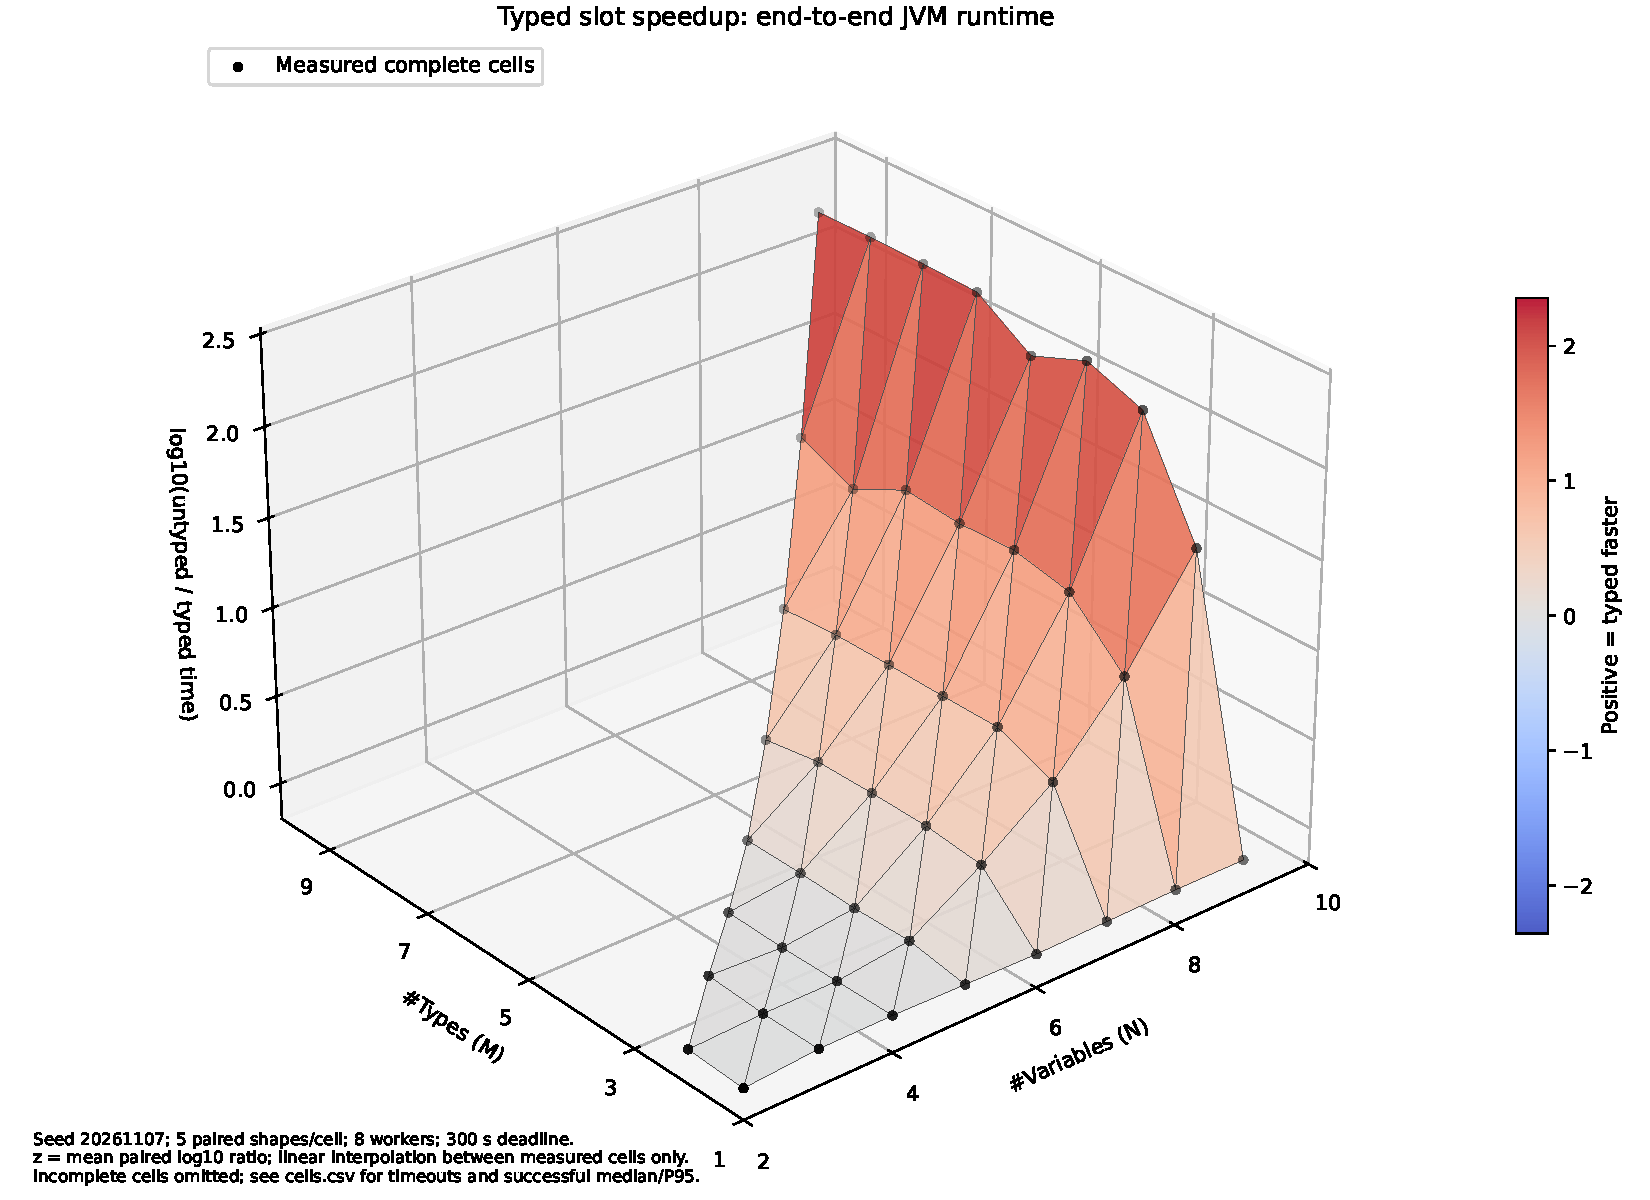
\includegraphics[width=0.78\linewidth]{figures/wall-speedup-surface.pdf}
\caption{Synthetic typed-versus-untyped end-to-end JVM speedup surface
($\log_{10}$ ratio across the 44/54 complete matched cells, without
interpolating across censored timeout cells). Complements
Figure~\ref{fig:synthetic-grid}.}
\label{fig:synthetic-wall-surface}
\end{figure}

\subsection{Bounded Semantic Validation Checks}

The natural checker evaluated 4,499 distinct zero
claims in the source models and found no counterexamples at the recorded
bounds. Each of the four deliberately invalid probes was refused by all
seven ablation arms. The capability study ran 29 bounded
sample checks across the generated families.

\subsection{Reproduction Identifiers}

\begingroup
\def\UrlBreaks{\do\-\do\_\do\/\do0\do1\do2\do3\do4\do5\do6\do7\do8\do9%
  \do\a\do\b\do\c\do\d\do\e\do\f}
\Urlmuskip=0mu plus 1mu\relax
The v3.3 experiment froze commit \path{d5c0c2a07504d53b13b28c61e9e64768c37eb984}.
It used 16 workers, an 8\,GiB heap cap, reward pool 100 and seed
\texttt{55520260811}. The following identifiers preserve the v3 synthetic
and historical study configuration.
\begin{itemize}
\item Experiment commit: \path{2d70f89ab67241cd071387ecedd3b2f432821921}.
\item Release commit (tag \texttt{v3}): \path{8770cb4b5f7133bad78058d9bc214f0ca36130d0}.
\item Natural corpus SHA-256 (66,080 files):
  \path{d6741fbf4c4a9b3714d012d068f84cc918052f1f55211bf4d0443b990736a689}.
\item Synthetic scaling dataset SHA-256 (270 pairs / 540 predicates):
  \path{c490b2bb1e6199f2ed221aa3f1b2d22b1da5dd8604341f305302c27a45de6b5f}.
\item Rule set: \texttt{canonical-equivalences-v3-explicit-laws};\\
  repair metric manifest ID:\\
  \texttt{certified-fast-rewrite-repair-distance-v25-}\\
  \texttt{retained-phase-representation}.
\item Natural and capability environment: AMD Ryzen~9 9950X3D (32 logical
  processors), OpenJDK~17.0.21.0.3, 16 workers, 8\,GiB heap, seed
  \texttt{55520260811}. Natural ablation run ID:
  \path{8dfc4fcc-84f0-4e9e-a88f-218fe05439b6}.
\item Synthetic grid environment: 8 concurrent isolated JVMs, 768\,MiB heap per
  JVM, 300-second deadline per predicate per arm; run ID:
  \path{e3d9bc4e-a514-471b-9e01-162562663f2e}.
\end{itemize}
\endgroup

\clearpage
\section{Rewrite Policy and Side Conditions}
\label{app:canon-rules}

Section~\ref{sec:canonicalization-procedure} describes canonical-record
construction. This appendix collects the rewrite choices used to expose and
normalize operands. A rule applies only to a typed operator instance whose side
conditions hold; the resulting source equation supplies the local certificate
consumed by the soundness argument.

\subsection{Rewrite Order and Side Conditions}
\label{app:rule-order}

The normalization order is parser cleanup, alpha normalization,
capture-avoiding let substitution, branch elimination, negation normalization,
phase-local prenexing and domain guarding, repeated negation and neutral
cleanup after unused-binding removal, membership elimination prior to
destructive distribution, container normalization, and local saturation with
rebuilding. Quantifier motion stays within a temporal phase unless an explicit
source law permits crossing its boundary.

Parser aliases share an internal head only when the frontend establishes the
same operator and type instance. Let substitution avoids capture via lifted de
Bruijn substitution, which preserves newly introduced bound positions while
substituting into outer scopes.

\paragraph{Boolean rules.}
Branch elimination uses
\begin{align*}
 A\Rightarrow B&=\neg A\lor B,\\
 A\Leftrightarrow B&=(\neg A\lor B)\land(\neg B\lor A),\\
 \operatorname{ite}(C,A,B)&=(C\land A)\lor(\neg C\land B)
\end{align*}
for formula-valued conditionals. Negation normalization applies double
negation, constant negation, and De Morgan's laws. Local saturation adds
Boolean identities, annihilators, idempotence, and complements:
\begin{align*}
 A\land\top&=A,& A\lor\bot&=A,&
 A\land\bot&=\bot,& A\lor\top&=\top,\\
 A\land A&=A,& A\lor A&=A,&
 A\land\neg A&=\bot,& A\lor\neg A&=\top.
\end{align*}
Recognizing complementary atoms requires equality of the underlying normalized
atoms, not merely matching operator names. Empty or singleton containers reduce
to units or children only when the operator's laws license those endpoints.

\paragraph{Temporal and atomic duals.}
Negation exchanges always/eventually, historically/once, until/releases, and
since/triggered with negated operands under the intended temporal semantics.
Atomic duals include equality/inequality, membership/nonmembership, and
complementary comparisons; unsupported operators keep an explicit negation.

\paragraph{Quantifiers, domains, and scheduling.}
Universal and existential negation swap the quantifier and negate the body,
while multiplicity quantifiers use their own duals (e.g., negating
\textsf{one} yields \textsf{notone}). Empty-domain laws handle each quantifier
explicitly: \textsf{all}, \textsf{no}, and \textsf{lone} over an empty domain
are true, whereas \textsf{some} and \textsf{one} are false. For finite
carriers $C$, predicates $p,d$, and $r$ independent of the bound variable,
\begin{align*}
 (\exists_C p)\land r&=\exists_C(\lambda x.\,p(x)\land r),&
 \exists_{\operatorname{filter}(d,C)}p&=\exists_C(\lambda x.\,d(x)\land p(x)),\\
 (\forall_C p)\lor r&=\forall_C(\lambda x.\,p(x)\lor r),&
 \forall_{\operatorname{filter}(d,C)}p&=\forall_C(\lambda x.\,\neg d(x)\lor p(x)).
\end{align*}
These identities hold even when $C$ is empty, whereas other quantifier/connective
combinations may require nonemptiness and are not generalized by analogy.
Unused-binder removal is followed by neutral cleanup so equivalent subterms
reached by different simplification paths stabilize to the same shape, and
membership elimination on relations runs before destructive distribution so
source shapes needed by guarded rewrites are preserved.

Binder-block permutations must preserve the full descriptor—types, domains,
multiplicities, disjointness classes, and dependencies—rather than merely
permuting slots of matching types.

\subsection{Operator Profiles}

The Alloy operator profile assigns carriers as follows:
\begin{itemize}
\item Boolean conjunction and disjunction, and relational union and
  intersection, use $\Set$ ports with licensed flattening.
\item Integer addition and multiplication use $\Bag$ ports; flattening is
  licensed for modular $\operatorname{Fin}(2^w)$ arithmetic, whereas with
  overflow rejection $(7+1)+(-1)$ fails in signed 4-bit arithmetic while
  $7+(1+(-1))=7$, forbidding unguarded reassociation.
\item Equality, inequality, and biconditional use commutative binary ports
  without recursive flattening.
\item Relational join, product, calls, and total-order predicates retain
  positional ports; disjointness predicates use nonflat bags.
\end{itemize}
Under Alloy's subset semantics, $x\ \texttt{in}\ \texttt{none}$ reduces to false
only when $x$ is known nonempty, since an empty relation is a subset of
\texttt{none}. Finally, canonical equality ($d=0$ under a complete finite
presentation) tests membership in the declared structural quotient, whereas
repair distance ($d_{\mathrm{repair}}>0$) measures structural edits between
repair projections; Section~\ref{sec:evaluation} reports them separately.

\end{document}
